% !TeX program = xelatex
\RequirePackage{fix-cm}
\documentclass[14pt,a4paper]{extarticle}
\usepackage{fontspec}
\defaultfontfeatures{Ligatures=TeX}
\input{build/font-path.tex}
\ifdefined\reportFontPath
  \setmainfont{Times.TTF}[Path=\reportFontPath,BoldFont=Timesbd.TTF,ItalicFont=Timesi.TTF,BoldItalicFont=Timesbi.TTF]
  \newfontfamily\cyrillicfont{Times.TTF}[Path=\reportFontPath,BoldFont=Timesbd.TTF,ItalicFont=Timesi.TTF,BoldItalicFont=Timesbi.TTF,Script=Default]
\else
  \setmainfont{Times New Roman}
  \newfontfamily\cyrillicfont{Times New Roman}
\fi
\setmonofont{FreeMono}
\newfontfamily\cyrillicfonttt{FreeMono}
\usepackage{polyglossia}
\setdefaultlanguage{russian}
\setotherlanguage{english}
\usepackage[left=30mm,right=10mm,top=20mm,bottom=20mm,footskip=10mm]{geometry}
\usepackage{setspace}
\makeatletter
\renewcommand{\normalsize}{\@setfontsize\normalsize{14bp}{16.8bp}}
\makeatother
\onehalfspacing
\AtBeginDocument{\normalsize}
\setlength{\parindent}{1.25cm}
\setlength{\parskip}{0pt}
\usepackage{indentfirst}
\usepackage{array,tabularx,graphicx,float,caption,fvextra,xcolor}
\DeclareCaptionLabelSeparator{gost}{~—~}
\captionsetup{font=small,labelsep=gost,justification=centering,singlelinecheck=false}
\captionsetup[table]{justification=raggedright,position=top,skip=6pt}
\captionsetup[figure]{skip=8pt}
\addto\captionsrussian{\renewcommand{\figurename}{Рисунок}\renewcommand{\tablename}{Таблица}}
\usepackage{titlesec}
\titleformat{\section}[block]{\normalfont\bfseries\centering}{\thesection.}{.5em}{\MakeUppercase}
\titlespacing*{\section}{0pt}{0pt}{18pt}
\usepackage{enumitem}
\usepackage{xurl}
\urlstyle{same}
\usepackage[hidelinks,unicode,pdfauthor={Матвеев М. А.},pdftitle={Лабораторная работа №4. Элементы формы}]{hyperref}
\pagestyle{plain}
\emergencystretch=2em
\clubpenalty=10000
\widowpenalty=10000
\raggedbottom
\newcolumntype{Y}{>{\raggedright\arraybackslash}X}
\newcommand{\code}[1]{{\fontsize{12}{14}\selectfont\texttt{#1}}}
\input{build/highlight-style.tex}
\newcommand{\listing}[1]{\begingroup\singlespacing\setlength{\topsep}{0pt}\setlength{\partopsep}{0pt}\input{build/#1.tex}\endgroup}

\begin{document}
\begin{titlepage}
\thispagestyle{empty}
\begin{center}
\bfseries
МИНОБРНАУКИ РОССИИ\\
Федеральное государственное автономное\\
образовательное учреждение высшего образования\\
«Санкт-Петербургский государственный\\
электротехнический университет «ЛЭТИ»\\
им. В.И. Ульянова (Ленина)»\\
Кафедра информационных систем
\end{center}
\vspace{30mm}
\begin{center}
\textbf{ОТЧЕТ ПО ЛАБОРАТОРНОЙ РАБОТЕ №4}\\[8mm]
«Элементы формы»
\end{center}
\vfill
\noindent\begin{tabularx}{\textwidth}{@{}lXr@{}}
Студент гр. 4372 & \centering\rule{25mm}{0.3pt} & Матвеев М. А.\\[8mm]
Преподаватель & \centering\rule{25mm}{0.3pt} & Нечитайленко Р. А.\\
\end{tabularx}
\vspace{20mm}
\begin{center}
Санкт-Петербург\\
2026
\end{center}
\end{titlepage}
\setcounter{page}{2}

\section{Цель и выполнение работы}
Цель работы: сверстать форму обратной связи по образцу.

Форма содержит имя и фамилию, адрес, город, регион, почтовый индекс, email, телефон, сообщение и флажок подписки. Связанные поля объединены элементом \code{fieldset} с заголовком \code{legend}. Атрибут \code{aria-label} задаёт доступные имена полей ввода и сообщения.

В широком окне имя и фамилия, а также email и телефон образуют пары. Город, регион и индекс расположены в три колонки. При ширине до 420~px поля выстраиваются в одну колонку.
\begin{figure}[H]
\centering
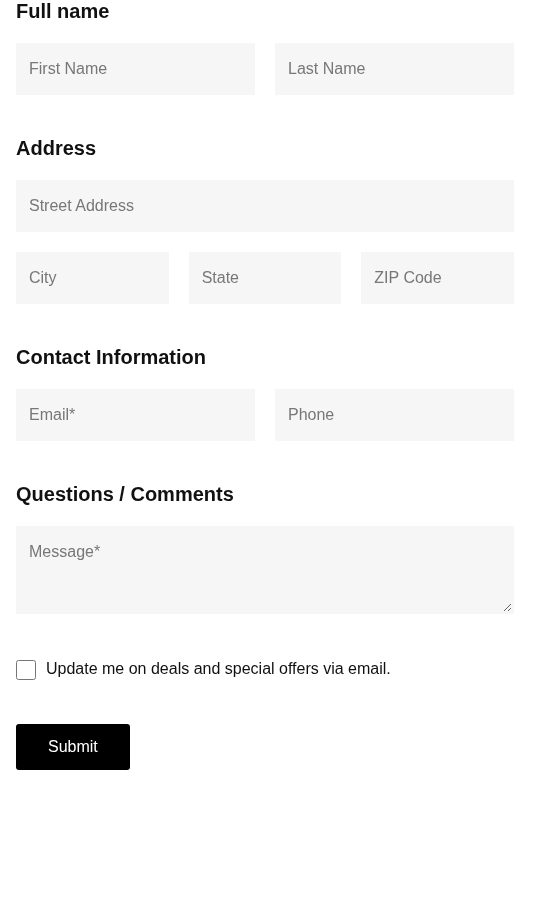
\includegraphics[width=\textwidth,height=155mm,keepaspectratio]{assets/desktop.png}
\caption{Форма обратной связи}
\end{figure}

\clearpage
\section{Элементы формы}
Для email задан \code{type="email"}, для телефона \code{type="tel"}, для сообщения используется \code{textarea}. Email и сообщение обязательны. Атрибуты \code{autocomplete} задают назначение полей для автозаполнения.

Подсказки в полях заданы атрибутом \code{placeholder}. Элемент \code{label} связывает текст подписки с флажком: нажатие на текст переключает его. Для перехода между полями используется клавиша Tab, активный элемент выделяется рамкой.

Кнопка Submit запускает встроенную проверку браузера. Пустые обязательные поля и неверный email блокируют отправку. При корректном вводе обработчик \code{submit} вызывает \code{preventDefault()}. Значения остаются в полях, сетевой запрос не выполняется.


\clearpage
\section{Исходный код: index.html}
\listing{index.html}

\vspace{4mm}
\noindent\begin{minipage}{\textwidth}
\section{Исходный код: script.js}
\listing{script.js}
\end{minipage}

\clearpage
\section{Исходный код: style.scss}
\listing{style.scss}

\clearpage
\section*{Список использованных источников}
\begin{enumerate}[label=\arabic*.,leftmargin=8mm,itemsep=8pt,parsep=0pt]
\item Тег <form> // HTMLbook.ru. URL: \url{https://htmlbook.ru/html/form}.
\item Тег <fieldset> // HTMLbook.ru. URL: \url{https://htmlbook.ru/html/fieldset}.
\item Атрибут type // HTMLbook.ru. URL: \url{https://htmlbook.ru/html/input/type}.
\item Тег <textarea> // HTMLbook.ru. URL: \url{https://htmlbook.ru/html/textarea}.
\item Атрибут required // HTMLbook.ru. URL: \url{https://htmlbook.ru/html/input/required}.
\item Dart Sass Command-Line Interface // Sass. URL: \url{https://sass-lang.com/documentation/cli/dart-sass/}.
\end{enumerate}
\end{document}
